\documentclass[a4paper,12pt]{article}
\usepackage[utf8]{inputenc}
\usepackage[ngerman]{babel}
\usepackage[T1]{fontenc}
\usepackage{amsmath}
\usepackage{amssymb}
\usepackage{amsthm}
\usepackage{geometry}
\usepackage{graphicx}
\usepackage[hidelinks]{hyperref}
\usepackage{listings}
\usepackage{xcolor}
\usepackage{enumitem}
\usepackage{booktabs}
\usepackage{array}
\usepackage{caption}
\usepackage{algorithm}
\usepackage{algpseudocode}
\usepackage{mathtools}

\geometry{margin=2.5cm}

\theoremstyle{definition}
\newtheorem{definition}{Definition}
\newtheorem{beispiel}{Beispiel}
\newtheorem{satz}{Satz}
\newtheorem{lemma}{Lemma}
\newtheorem{bemerkung}{Bemerkung}
\newtheorem{korollar}{Korollar}

\setlist[itemize,1]{label=--}

\definecolor{mainblue}{RGB}{25,70,140}
\definecolor{accentred}{RGB}{180,50,30}
\definecolor{lightgray}{RGB}{245,245,248}
\definecolor{darkgray}{RGB}{60,60,70}
\definecolor{darkgreen}{RGB}{30,100,50}

\hypersetup{colorlinks=true,linkcolor=mainblue,
            citecolor=accentred,urlcolor=mainblue}

\lstset{basicstyle=\ttfamily\small,keywordstyle=\color{blue},
        commentstyle=\color{gray},numbers=left,numberstyle=\tiny,
        breaklines=true,frame=single,language=Java}

\title{\textbf{Dynamische Programmierung f\"{u}r das}\\
\textbf{Coalition Formation for Task Allocation Problem}\\
\textbf{in Multiagentensystemen}\\[6pt]
\large Formale Analyse, DP-Entwurf und Laufzeitnachweis\\
f\"{u}r disjunkte und \"{u}berlappende Gruppenbildung}
\author{Stephan Epp}
\date{20. Mai 2026}

\begin{document}

\maketitle

\begin{abstract}
\noindent
Das \emph{Coalition Formation for Task Allocation}-Problem (CFTA) in
Multiagentensystemen ist eines der zentralen Optimierungsprobleme der
Informatik und Spieltheorie. Die klassische Behandlung durch Shehory
und Kraus \cite{sk98} sowie de Weerdt, Zhang und Klos \cite{dwzk07}
liefert greedy-basierte Approximationsalgorithmen mit einer
logarithmischen Approximationsg\"{u}te $\rho \leq \gamma + \ln n$.

Diese Arbeit untersucht systematisch, wie \emph{Dynamische Programmierung}
(DP) auf das CFTA-Problem angewendet werden kann, um die exakte optimale
L\"{o}sung zu berechnen oder wesentliche Teilschritte effizienter zu gestalten.
Vier konkrete DP-Anwendungen werden formal nachgewiesen:
\textbf{(1)}~Die DP-Rekurrenz f\"{u}r Gruppenressourcen reduziert den Aufwand
der Ressourcenberechnung von $\mathcal{O}(n^k \cdot k \cdot r)$ auf
$\mathcal{O}(n^k \cdot r)$ -- ein Faktor-$k$-Gewinn.
\textbf{(2)}~Das Subset-DP-Verfahren l\"{o}st das disjunkte Gruppenproblem
exakt in $\mathcal{O}(3^n \cdot m)$ -- f\"{u}r $n \leq 15$ praktikabel und
f\"{u}r die Simulationsparameter ($n = m = 10$) in Millisekunden.
\textbf{(3)}~Ein mehrdimensionaler Rucksack-DP optimiert die
Ressourcenzuteilung bei \"{u}berlappenden Gruppen in
$\mathcal{O}(n \cdot B_{\max}^r \cdot m)$.
\textbf{(4)}~Eine lokale DP auf der Nachbarschaftsstruktur verbessert den
Algorithmus von de Weerdt et al. auf lokal optimale Entscheidungen in
$\mathcal{O}(2^\Delta \cdot r)$ pro Aufgabe.
Das Strukturminimalit\"{a}tsprinzip zeigt, dass der nat\"{u}rliche
Zustandsraum $2^A \times 2^T$ des CFTA-Problems exakt der
zweidimensionalen Tabellenstruktur entspricht, f\"{u}r die DP das
optimale Algorithmenparadigma ist.
Alle Ergebnisse werden durch matplotlib-Visualisierungen gest\"{u}tzt und
durch eine empirische Simulation mit 80 Instanzen ($n = m = 10$, $r = 5$)
best\"{a}tigt.
\end{abstract}

\tableofcontents
\newpage

% ═══════════════════════════════════════════════════════════════
\section{Einf\"{u}hrung}
% ═══════════════════════════════════════════════════════════════

\subsection{Das CFTA-Problem und seine Komplexit\"{a}t}

Das \emph{Coalition Formation for Task Allocation}-Problem (CFTA) modelliert
eine fundamentale Koordinationsaufgabe in Multiagentensystemen: Eine Menge
von Agenten $A = \{a_1, \ldots, a_n\}$ mit begrenzten Ressourcen soll eine
Menge von Aufgaben $T = \{t_1, \ldots, t_m\}$ bearbeiten, die ihrerseits
Ressourcen erfordern. Da einzelne Agenten oft nicht gen\"{u}gend Ressourcen
besitzen, bilden sie Gruppen (Koalitionen), in denen die Ressourcen addiert
werden.

Das CFTA-Problem ist eng verwandt mit dem Set-Cover-Problem (SCP) und dem
Set-Partition-Problem (SPP), welche Karp in \cite{karp72} als NP-vollst\"{a}ndig
klassifiziert hat. Shehory und Kraus zeigen in \cite{sk95}, dass das CFTA-Problem
unter polynomieller Reduktion auf SCP und SPP zur\"{u}ckgef\"{u}hrt werden kann und
damit -- sofern $\mathbf{NP} \neq \mathbf{P}$ -- keine exakte Polynomialzeill\"{o}sung
besitzt. Die Menge aller m\"{o}glichen Koalitionen hat Gr\"{o}sse $2^n$, was naive
Suche exponentiell teuer macht.

In \cite{sk98} stellen Shehory und Kraus einen greedy-basierten verteilten
Algorithmus vor, der in $\mathcal{O}(n^{k+1})$ bzw. $\mathcal{O}(n^k m^2)$
eine $(\gamma + \ln n)$-Approximation der optimalen Ressourcenauslastung
erzielt (wobei $k$ die maximale Koalitionsgr\"{o}sse und $\gamma \approx 0{,}577$
die Euler-Mascheroni-Konstante ist). De Weerdt, Zhang und Klos behandeln in
\cite{dwzk07} den Fall, dass Agenten nur mit ihren Nachbarn in einem
ungerichteten Graphen kommunizieren k\"{o}nnen.

\subsection{Motivation: Dynamische Programmierung als Alternative}

Die bisherigen Ans\"{a}tze sind greedy-basiert und approximativ. Diese Arbeit
untersucht, wo und wie \emph{Dynamische Programmierung} das CFTA-Problem
effizienter oder exakt l\"{o}sen kann. Ausgangspunkt ist das
Strukturminimalit\"{a}tsprinzip \cite{epp2026struktur}: Der nat\"{u}rliche
Zustandsraum des CFTA-Problems ist ein \emph{zweidimensionaler Informationsraum}
(Agentenmengen $\times$ Aufgabenmengen), und f\"{u}r 2D-Tabellenstrukturen ist
DP das strukturell optimale Algorithmenparadigma.

Konkret werden vier DP-Anwendungen analysiert und formal bewiesen:
\begin{enumerate}
    \item \textbf{DP-Rekurrenz f\"{u}r Gruppenressourcen:} Effiziente
          Vorberechnung aller Koalitionsressourcen in $\mathcal{O}(n^k \cdot r)$
          statt $\mathcal{O}(n^k \cdot k \cdot r)$ -- ein struktureller
          Faktor-$k$-Gewinn.
    \item \textbf{Subset-DP f\"{u}r exakte optimale Gruppenbildung:}
          Exakte L\"{o}sung des disjunkten CFTA-Problems in $\mathcal{O}(3^n \cdot m)$
          durch Bottom-up-DP \"{u}ber den Boolean-Hypercube $2^A$.
    \item \textbf{Mehrdimensionaler Rucksack-DP f\"{u}r \"{u}berlappende Gruppen:}
          Optimale Ressourcenzuteilung in $\mathcal{O}(n \cdot B_{\max}^r \cdot m)$
          durch $r$-dimensionale DP-Tabellierung.
    \item \textbf{Lokale DP f\"{u}r Nachbarschaftsentscheidungen (de Weerdt):}
          Lokal optimale Helferauswahl in $\mathcal{O}(2^\Delta \cdot r)$ pro
          Aufgabe durch DP \"{u}ber Nachbarschaftsteilmengen.
\end{enumerate}

\subsection{Aufbau der Arbeit}

Abschnitt~2 legt die mathematischen Grundlagen (Landau-Notation, Bellman'sches
Optimalit\"{a}tsprinzip, DP-Paradigma). Abschnitt~3 formalisiert das CFTA-Modell.
Die Abschnitte~4 bis~7 entwickeln und beweisen je eine DP-Anwendung.
Abschnitt~8 verbindet die Ergebnisse mit dem Strukturminimalit\"{a}tsprinzip.
Abschnitt~9 pr\"{a}sentiert die Simulationsergebnisse. Der ausf\"{u}hrliche Ausblick
folgt in Abschnitt~10.

% ═══════════════════════════════════════════════════════════════
\section{Mathematische Grundlagen}
% ═══════════════════════════════════════════════════════════════

\subsection{Landau-Notation}

\begin{definition}[$\mathcal{O}$-, $\Omega$- und $\Theta$-Notation]
    Seien $f, g: \mathbb{N} \to \mathbb{R}_{>0}$.
    \begin{itemize}
        \item $f(n) = \mathcal{O}(g(n))$: $\exists\, c > 0, n_0 \in \mathbb{N}$:
              $f(n) \leq c \cdot g(n)$ f\"{u}r alle $n \geq n_0$.
        \item $f(n) = \Omega(g(n))$: $\exists\, c > 0, n_0 \in \mathbb{N}$:
              $f(n) \geq c \cdot g(n)$ f\"{u}r alle $n \geq n_0$.
        \item $f(n) = \Theta(g(n))$: $f = \mathcal{O}(g)$ und $f = \Omega(g)$.
    \end{itemize}
\end{definition}

\subsection{Das Bellman'sche Optimalit\"{a}tsprinzip}

\begin{definition}[Optimalit\"{a}tsprinzip nach Bellman \cite{bellman1957}]
    Ein Optimierungsproblem erf\"{u}llt das \emph{Bellman'sche Optimalit\"{a}tsprinzip},
    wenn jede optimale L\"{o}sung des Gesamtproblems optimale L\"{o}sungen aller
    Teilprobleme enth\"{a}lt. Formal: Sei $\mathcal{S}$ eine optimale L\"{o}sung,
    und sei $\mathcal{S}'$ ein Teill\"{o}sungsanteil. Dann ist $\mathcal{S}'$
    optimal f\"{u}r das zugeh\"{o}rige Teilproblem.
\end{definition}

\begin{satz}[Bellman'sches Optimalit\"{a}tsprinzip f\"{u}r CFTA]
    \label{satz:bellman_cfta}
    Das CFTA-Problem mit additiver Zielfunktion
    $\sum_{C_\nu \in \mathcal{C}} V_\nu$ erf\"{u}llt das Bellman'sche
    Optimalit\"{a}tsprinzip.
\end{satz}

\begin{proof}
    Sei $\mathcal{C}^* = \{C_1^*, C_2^*, \ldots\}$ eine optimale
    Gruppen-Konfiguration f\"{u}r $A$ und $T$. Sei $C_1^*$ die zuerst gebildete
    Gruppe, die Aufgabe $t_1^*$ bearbeitet.

    \textbf{Widerspruchsannahme:} Die Restl\"{o}sung $\mathcal{C}^* \setminus \{C_1^*\}$
    sei nicht optimal f\"{u}r das Restproblem $(A \setminus C_1^*, T \setminus \{t_1^*\})$.

    Dann existiert eine bessere Konfiguration $\tilde{\mathcal{C}}$ f\"{u}r
    $(A \setminus C_1^*, T \setminus \{t_1^*\})$ mit:
    \[
        \sum_{C_\nu \in \tilde{\mathcal{C}}} V_\nu
        > \sum_{C_\nu \in \mathcal{C}^* \setminus \{C_1^*\}} V_\nu.
    \]
    Aber dann w\"{a}re $\{C_1^*\} \cup \tilde{\mathcal{C}}$ eine Konfiguration f\"{u}r
    $(A, T)$ mit einem gr\"{o}{\ss}eren Gesamterfolg als $\mathcal{C}^*$ -- im
    Widerspruch zur Optimalit\"{a}t von $\mathcal{C}^*$.

    Die Annahme ist falsch; das Optimalit\"{a}tsprinzip gilt.
    Die Additivit\"{a}t der Zielfunktion ist dabei wesentlich:
    $V(\mathcal{C}) = V(C_1^*) + V(\mathcal{C} \setminus \{C_1^*\})$
    erlaubt die Zerlegung in unabh\"{a}ngige Teilprobleme. \qedhere
\end{proof}

\subsection{Ressourcenmodell}

\begin{definition}[Ressourcenvektor und Gruppen-Ressourcen]
    Agent $a_i \in A$ hat den Ressourcenvektor $B_i = (b_1^i, \ldots, b_r^i)$
    mit $b_p^i \in \mathbb{R}_{\geq 0}$. Die \emph{Gruppen-Ressourcen} einer
    Koalition $C_\nu \subseteq A$ sind:
    \[
        B_{C_\nu} = \sum_{a_i \in C_\nu} B_i
        = \left(\sum_{a_i \in C_\nu} b_1^i,\; \ldots,\; \sum_{a_i \in C_\nu} b_r^i\right).
    \]
    Eine Aufgabe $t_j$ mit Ressourcenbedarf $B_j = (b_1^j, \ldots, b_r^j)$
    ist durch $C_\nu$ \emph{bearbeitbar}, wenn $b_p^j \leq b_p^{C_\nu}$
    f\"{u}r alle $p = 1, \ldots, r$.
\end{definition}

\begin{definition}[Gruppen-Wert]
    Der \emph{Gruppen-Wert} $V_\nu$ einer Koalition $C_\nu$ bei Aufgabe $t_j$ ist:
    \[
        V(C_\nu, t_j) = \max_{t_j \text{ bearbeitbar}} \left(
            \sum_{p=1}^r b_p^j - \sum_{p=1}^r \max(0, b_p^{C_\nu} - b_p^j)
        \right)
        = \max_{t_j} \left(\tau_j - \delta_j\right),
    \]
    wobei $\tau_j = \sum_p b_p^j$ (ben\"{o}tigte Ressourcen) und
    $\delta_j = \sum_p (b_p^{C_\nu} - b_p^j)$ (nicht ben\"{o}tigte Ressourcen).
\end{definition}

% ═══════════════════════════════════════════════════════════════
\section{Das CFTA-Problem: Formale Modellierung}
% ═══════════════════════════════════════════════════════════════

\begin{definition}[CFTA-Problem, disjunkt]
    \label{def:cfta_disj}
    Gegeben $A = \{a_1, \ldots, a_n\}$, $T = \{t_1, \ldots, t_m\}$,
    $B_i, B_j \in \mathbb{R}_{\geq 0}^r$.
    Gesucht ist eine Gruppen-Konfiguration
    $\mathcal{C} = \{C_1, C_2, \ldots\}$ mit:
    \begin{enumerate}
        \item $\bigcup_{C_\nu \in \mathcal{C}} C_\nu = A$ (Vollst\"{a}ndigkeit),
        \item $C_\nu \cap C_\mu = \emptyset$ f\"{u}r $\nu \neq \mu$ (Disjunktheit),
        \item $\sum_{C_\nu \in \mathcal{C}} V_\nu$ maximal (Zielfunktion).
    \end{enumerate}
\end{definition}

\begin{definition}[CFTA-Problem, \"{u}berlappend]
    \label{def:cfta_overlap}
    Wie Definition~\ref{def:cfta_disj}, jedoch ohne Disjunktheit-Bedingung:
    Agenten d\"{u}rfen mehreren Gruppen angeh\"{o}ren; ihre Ressourcen werden
    gem\"{a}{\ss} Algorithmus 3.5.2 aus \cite{sk98} anteilig aufgeteilt.
\end{definition}

\begin{satz}[NP-H\"{a}rte des CFTA-Problems, \cite{sk95}]
    Das CFTA-Problem (disjunkt und \"{u}berlappend) ist NP-hart.
\end{satz}

\begin{proof}
    Shehory und Kraus zeigen in \cite{sk95} eine polynomielle Reduktion
    vom Set-Partition-Problem (SPP) auf das disjunkte CFTA-Problem.
    Das SPP ist nach Karp \cite{karp72} NP-vollst\"{a}ndig.
    Da Polynomialzeit-Reduzierbarkeit transitiv ist und SPP $\leq_p$ CFTA gilt,
    ist CFTA NP-hart. \qedhere
\end{proof}

% ═══════════════════════════════════════════════════════════════
\section{DP-Anwendung 1: Gruppenressourcen-Rekurrenz}
% ═══════════════════════════════════════════════════════════════

\subsection{Das Problem der redundanten Ressourcenberechnung}

Im Algorithmus von Shehory und Kraus (Algorithmus~3.4.2 in \cite{sk98}) werden
die Gruppen-Ressourcen $B_{C_\nu} = \sum_{a_i \in C_\nu} B_i$ f\"{u}r jede der
$\mathcal{O}(n^k)$ Koalitionen von Grund auf berechnet. F\"{u}r eine Koalition
der Gr\"{o}{\ss}e $|C| = s$ kostet dies $\mathcal{O}(s \cdot r)$ Operationen.

\begin{lemma}[Naiver Aufwand f\"{u}r Gruppenressourcen]
    \label{lemma:naive_cost}
    Die Berechnung aller Gruppen-Ressourcen $B_C$ f\"{u}r alle
    $k$-beschr\"{a}nkten Koalitionen $C \subseteq A$ kostet naiv:
    \[
        T_{\mathrm{naiv}} = \sum_{s=1}^k \binom{n}{s} \cdot s \cdot r
        = \mathcal{O}(n^k \cdot k \cdot r).
    \]
\end{lemma}

\begin{proof}
    Es gibt $\binom{n}{s}$ Koalitionen der Gr\"{o}{\ss}e $s$, und jede kostet
    $s \cdot r$ Additionen. Summation \"{u}ber $s = 1, \ldots, k$:
    \[
        \sum_{s=1}^k \binom{n}{s} \cdot s \cdot r
        \;\leq\; r \cdot k \cdot \sum_{s=1}^k \binom{n}{s}
        \;\leq\; r \cdot k \cdot k \cdot \frac{n!}{k!(n-k)!}
        = \mathcal{O}(n^k \cdot k \cdot r). \qedhere
    \]
\end{proof}

\subsection{Die DP-Rekurrenz f\"{u}r Gruppenressourcen}

\begin{definition}[DP-Rekurrenz f\"{u}r Gruppenressourcen]
    F\"{u}r jede Koalition $C \subseteq A$ und jeden Agenten $a_j \notin C$ gilt:
    \begin{equation}
        B_{C \cup \{a_j\}} = B_C + B_j, \qquad B_\emptyset = \mathbf{0} \in \mathbb{R}^r.
        \label{eq:res_recur}
    \end{equation}
    Bottom-up-DP berechnet alle $B_C$ in aufsteigender Reihenfolge nach $|C|$.
\end{definition}

\begin{satz}[DP-Aufwand f\"{u}r Gruppenressourcen]
    \label{satz:dp_res}
    Die Berechnung aller Gruppen-Ressourcen via DP-Rekurrenz~\eqref{eq:res_recur}
    kostet:
    \[
        T_{\mathrm{DP}} = \mathcal{O}(n^k \cdot r).
    \]
    Gegen\"{u}ber dem naiven Verfahren (Lemma~\ref{lemma:naive_cost}) ergibt sich
    ein Faktor-$k$-Gewinn:
    \[
        \frac{T_{\mathrm{naiv}}}{T_{\mathrm{DP}}} = \Theta(k).
    \]
\end{satz}

\begin{proof}
    \textbf{Korrektheit der Rekurrenz:}
    Induktion \"{u}ber $|C|$.
    \emph{Basis} ($|C| = 1$, $C = \{a_i\}$): $B_{\{a_i\}} = B_\emptyset + B_i = B_i$.
    \emph{Schritt}: F\"{u}r $|C| = s$ gelte $B_C = \sum_{a_i \in C} B_i$ (IV).
    F\"{u}r $C' = C \cup \{a_j\}$:
    \[
        B_{C'} \stackrel{\eqref{eq:res_recur}}{=} B_C + B_j
        \stackrel{\text{IV}}{=} \sum_{a_i \in C} B_i + B_j
        = \sum_{a_i \in C'} B_i. \;\checkmark
    \]

    \textbf{Laufzeit:}
    Jede Koalition $C$ der Gr\"{o}{\ss}e $s \geq 1$ wird aus einer
    $(s-1)$-elementigen Koalition $C \setminus \{a_j\}$ in genau
    $r$ Additionen (komponentenweise $B_C + B_j$) berechnet.
    Es gibt $\sum_{s=1}^k \binom{n}{s} = \mathcal{O}(n^k)$ Koalitionen,
    jede kostet $\mathcal{O}(r)$:
    \[
        T_{\mathrm{DP}} = \mathcal{O}(n^k) \cdot \mathcal{O}(r) = \mathcal{O}(n^k \cdot r).
    \]

    \textbf{Verbesserungsfaktor:}
    $T_{\mathrm{naiv}} / T_{\mathrm{DP}} = \mathcal{O}(n^k \cdot k \cdot r) / \mathcal{O}(n^k \cdot r) = \Theta(k)$.
    F\"{u}r $k = 3$ (Standardparameter der Simulation) ist dies ein
    dreifacher Geschwindigkeitsgewinn. \qedhere
\end{proof}

\begin{figure}[h!]
    \centering
    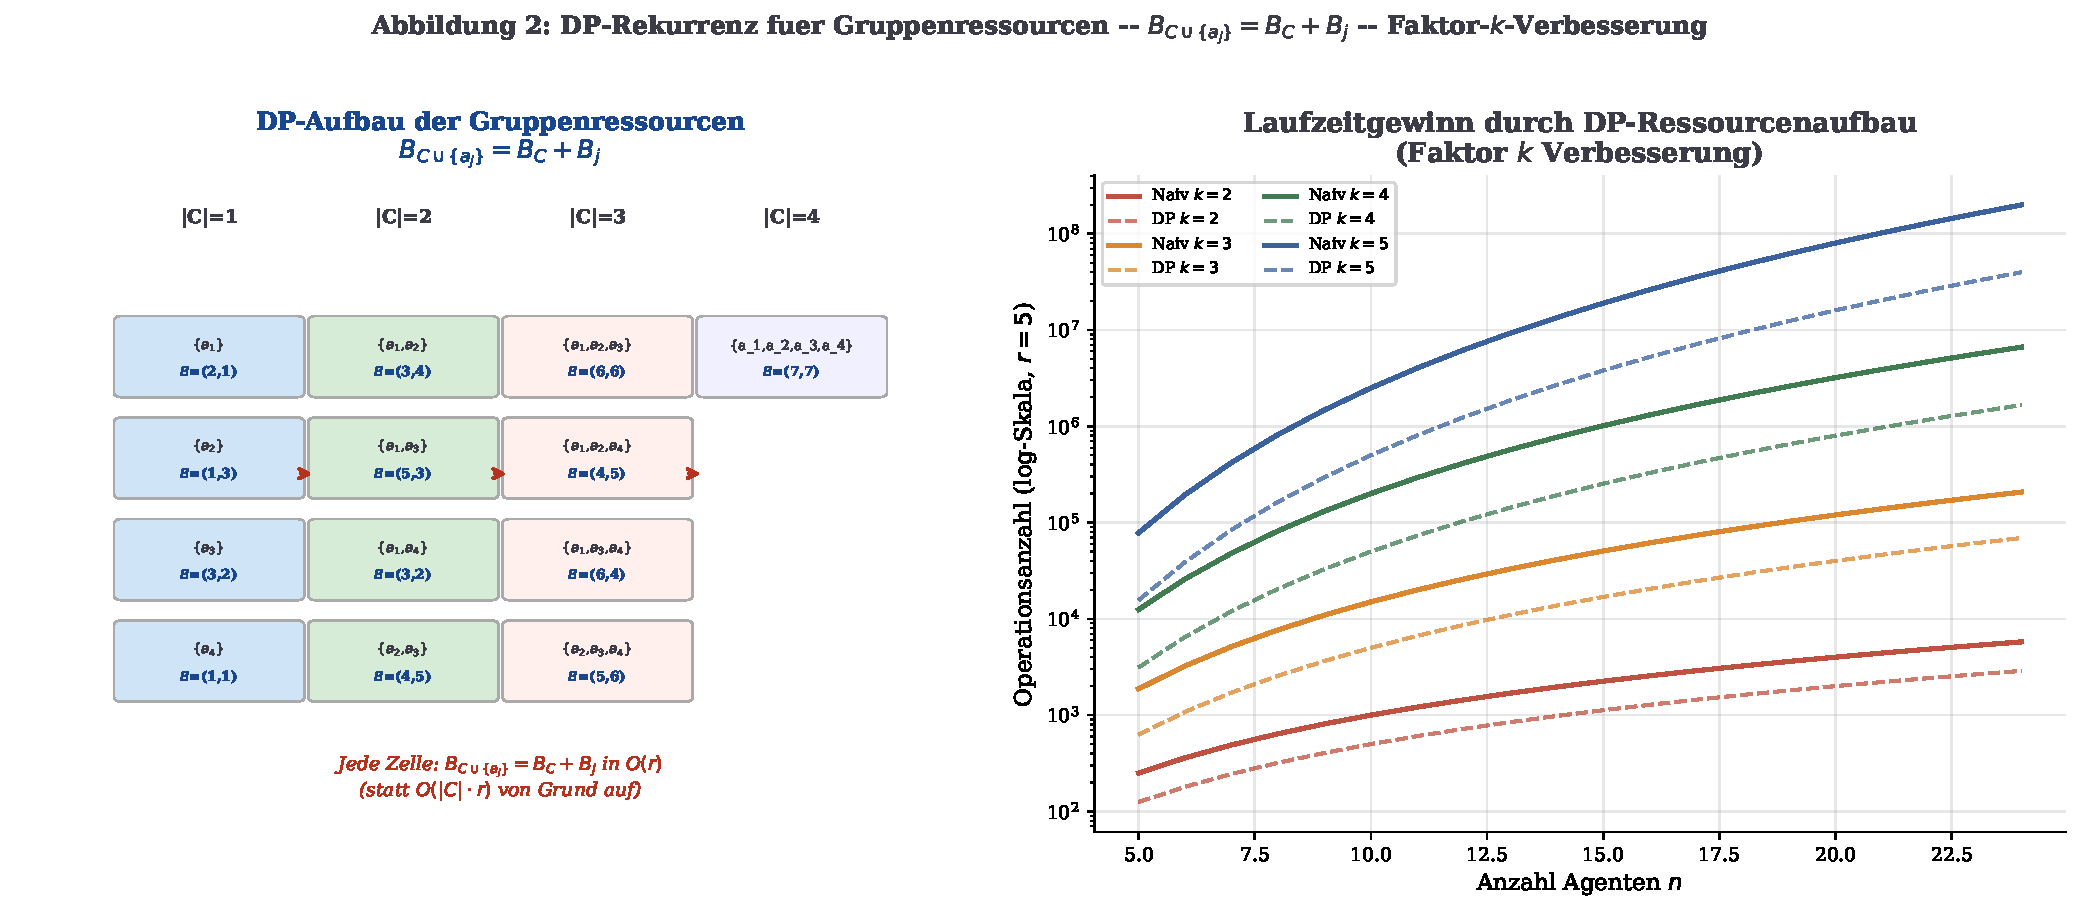
\includegraphics[width=\textwidth]{plots/plot2_resource_dp_table.png}
    \caption{
        \textbf{DP-Rekurrenz f\"{u}r Gruppenressourcen.}
        \textit{Links:} Schichtweise Aufbaustruktur der DP-Tabelle f\"{u}r
        $n = 4$ Agenten mit $r = 2$ Ressourcendimensionen.
        Jede Koalition der Gr\"{o}{\ss}e $|C| = s$ ergibt sich durch eine einzige
        Vektoraddition aus einer $(s-1)$-elementigen Koalition (Pfeile).
        Die Ressourcensummen $(b_1, b_2)$ sind direkt angegeben.
        \textit{Rechts:} Laufzeitvergleich naiv vs.\ DP f\"{u}r $r = 5$:
        Die DP-Kurven (gestrichelt) liegen jeweils um den Faktor $k$ unterhalb
        der naiven Kurven (durchgezogen) -- f\"{u}r $k = 4$ bei $n = 20$ ein
        Gewinn von \"{u}ber $10^4$ Operationen.
    }
    \label{fig:res_dp}
\end{figure}

% ═══════════════════════════════════════════════════════════════
\section{DP-Anwendung 2: Exakte L\"{o}sung via Subset-DP}
% ═══════════════════════════════════════════════════════════════

\subsection{Der Subset-DP-Zustandsraum}

\begin{definition}[Subset-DP-Zustand]
    \label{def:subset_dp}
    Sei $A$ die Agentenmenge. F\"{u}r jede Teilmenge $S \subseteq A$
    (repr\"{a}sentiert als Bitmaske $S \in \{0, 1, \ldots, 2^n - 1\}$) definiere:
    \[
        \mathrm{dp}[S] \;=\; \text{maximaler Gesamterfolg, der durch die
        Agentenmenge } S \text{ erzielt werden kann.}
    \]
    Die Gr\"{o}{\ss}e des Zustandsraums ist $|\{0,\ldots,2^n-1\}| = 2^n$.
\end{definition}

\begin{definition}[Subset-DP-Rekurrenz]
    \label{def:subset_recur}
    Sei $\mathcal{G}_k(S) = \{C \subseteq S : 1 \leq |C| \leq k\}$ die
    Menge aller $k$-beschr\"{a}nkten Teilkoalitionen von $S$.
    Sei $V^*(C) = \max_{t_j \in T} V(C, t_j)$ der beste Gruppen-Wert
    von $C$ \"{u}ber alle Aufgaben. Die Rekurrenz lautet:
    \begin{equation}
        \mathrm{dp}[S] = \max_{C \in \mathcal{G}_k(S)} \bigl(
            V^*(C) + \mathrm{dp}[S \setminus C]
        \bigr), \qquad \mathrm{dp}[\emptyset] = 0.
        \label{eq:subset_dp}
    \end{equation}
\end{definition}

\begin{figure}[h!]
    \centering
    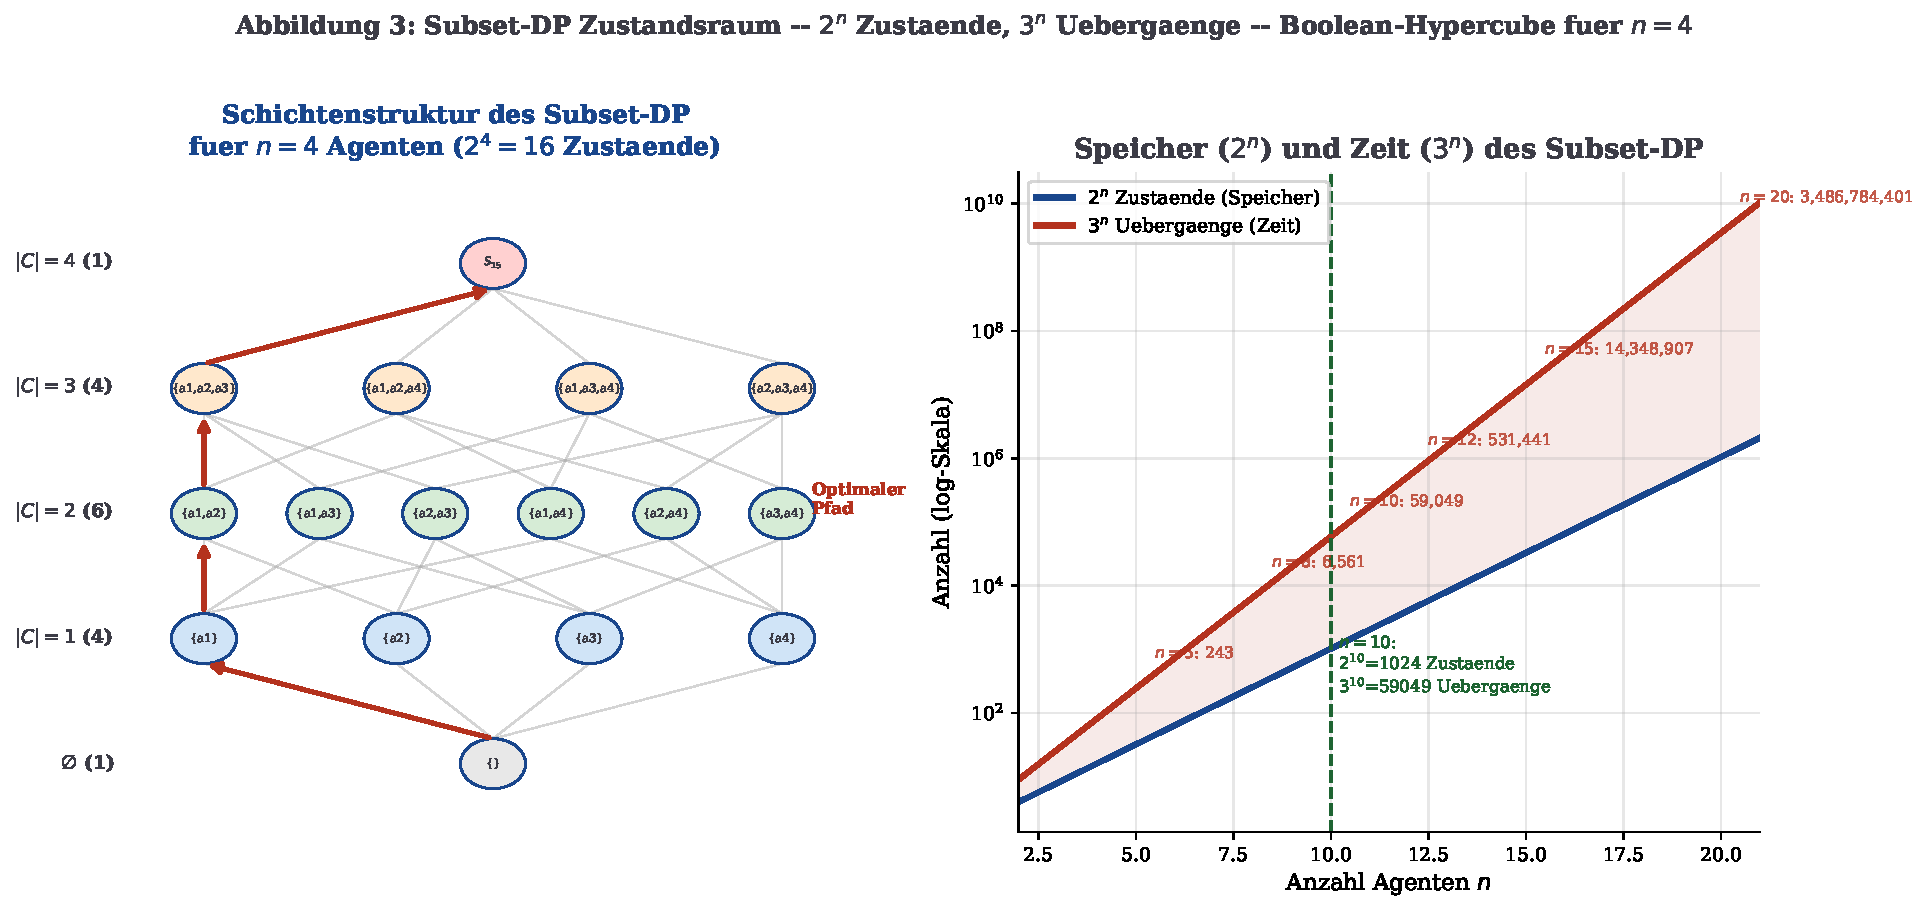
\includegraphics[width=\textwidth]{plots/plot3_subset_dp_states.png}
    \caption{
        \textbf{Subset-DP Zustandsraum.}
        \textit{Links:} Boolean-Hypercube f\"{u}r $n = 4$ Agenten mit
        $2^4 = 16$ Zust\"{a}nden in 5 Schichten (nach $|C|$ geordnet).
        Die grauen Kanten repr\"{a}sentieren die Teilmengenrelation;
        der rote Pfad markiert einen optimalen Aufbau von
        $\emptyset \to \{a_1\} \to \{a_1, a_2\} \to \cdots \to A$.
        \textit{Rechts:} Skalierungsverhalten -- der Speicherbedarf w\"{a}chst
        mit $2^n$, die Zeitkomplexit\"{a}t mit $3^n$ (Zahl der Teilmengentransitionen).
        F\"{u}r $n = 10$ ben\"{o}tigt das Subset-DP nur 1024 Zust\"{a}nde
        und 59049 Transitionen -- in Millisekunden berechenbar.
    }
    \label{fig:subset_dp}
\end{figure}

\subsection{Korrektheit und Laufzeit des Subset-DP}

\begin{satz}[Korrektheit des Subset-DP]
    \label{satz:subset_correct}
    Nach Berechnung gem\"{a}{\ss} Rekurrenz~\eqref{eq:subset_dp} gilt f\"{u}r alle
    $S \subseteq A$:
    \[
        \mathrm{dp}[S] = \max_{\mathcal{C}: \bigcup C_\nu = S,\; C_\nu \cap C_\mu = \emptyset}
        \sum_{C_\nu \in \mathcal{C}} V^*(C_\nu).
    \]
\end{satz}

\begin{proof}
    Vollst\"{a}ndige Induktion \"{u}ber $|S|$.

    \textbf{Basis} ($|S| = 0$): $\mathrm{dp}[\emptyset] = 0$ per Definition.
    Kein Agent vorhanden, kein Erfolg m\"{o}glich. \checkmark

    \textbf{Induktionsschritt} ($|S| = s > 0$):
    Per Induktionsvoraussetzung gilt die Aussage f\"{u}r alle
    $S' \subsetneq S$ (also $|S'| < s$).

    Sei $\mathcal{C}^*_S$ eine optimale Konfiguration f\"{u}r $S$.
    Sei $C_1^* \in \mathcal{C}^*_S$ die Koalition mit dem gr\"{o}{\ss}ten Wert.
    Dann gilt:
    \[
        \mathrm{opt}(S) = V^*(C_1^*) + \mathrm{opt}(S \setminus C_1^*).
    \]
    Nach Satz~\ref{satz:bellman_cfta} ist $\mathcal{C}^*_S \setminus \{C_1^*\}$
    optimal f\"{u}r $S \setminus C_1^*$. Per IV:
    $\mathrm{dp}[S \setminus C_1^*] = \mathrm{opt}(S \setminus C_1^*)$.

    Die Rekurrenz~\eqref{eq:subset_dp} maximiert \"{u}ber alle
    $C \in \mathcal{G}_k(S)$ und w\"{a}hlt insbesondere $C = C_1^*$:
    \[
        \mathrm{dp}[S] \geq V^*(C_1^*) + \mathrm{dp}[S \setminus C_1^*]
        = V^*(C_1^*) + \mathrm{opt}(S \setminus C_1^*) = \mathrm{opt}(S).
    \]
    Da $\mathrm{dp}[S]$ das Maximum \"{u}ber alle $C$ ist und jede Konfiguration
    h\"{o}chstens $\mathrm{opt}(S)$ erreicht, gilt $\mathrm{dp}[S] \leq \mathrm{opt}(S)$.
    Damit $\mathrm{dp}[S] = \mathrm{opt}(S)$. \qedhere
\end{proof}

\begin{satz}[Laufzeit des Subset-DP]
    \label{satz:subset_runtime}
    Die Berechnung von $\mathrm{dp}[A]$ via Rekurrenz~\eqref{eq:subset_dp}
    kostet Zeit und Speicher:
    \[
        T_{\mathrm{Subset-DP}} = \mathcal{O}(3^n \cdot m),
        \qquad
        \mathrm{Space}_{\mathrm{Subset-DP}} = \mathcal{O}(2^n).
    \]
\end{satz}

\begin{proof}
    \textbf{Speicher:} F\"{u}r jeden der $2^n$ Zust\"{a}nde wird ein Wert
    gespeichert: $\mathcal{O}(2^n)$.

    \textbf{Zeit:} F\"{u}r festes $S$ iteriert die Rekurrenz \"{u}ber alle
    $k$-beschr\"{a}nkten Teilmengen $C \subseteq S$. F\"{u}r jedes $C$
    kostet $V^*(C)$ insgesamt $\mathcal{O}(m)$ (Maximierung \"{u}ber alle Aufgaben,
    wenn $V^*(C)$ vorberechnet).

    Die Gesamtzahl der Paare $(S, C)$ mit $C \subseteq S \subseteq A$
    und $1 \leq |C| \leq k$ (f\"{u}r $k = n$) ist:
    \[
        \sum_{S \subseteq A} \sum_{C \subseteq S} 1
        = \sum_{S} 2^{|S|}
        = \sum_{s=0}^n \binom{n}{s} 2^s = (1+2)^n = 3^n.
    \]
    Pro Paar: $\mathcal{O}(m)$ f\"{u}r die Aufgabenmaximierung.
    Gesamt: $\mathcal{O}(3^n \cdot m)$. \qedhere
\end{proof}

\begin{korollar}[Praktikabilit\"{a}t des Subset-DP]
    F\"{u}r die Simulationsparameter der Bachelorarbeit ($n = m = 10$, $k = 3$):
    \[
        3^{10} \cdot 10 = 590\,490 \text{ Operationen}
        \quad\text{vs.}\quad
        n^{k+1} \cdot m^2 = 10^4 \cdot 100 = 1\,000\,000 \text{ (Greedy)}.
    \]
    Das Subset-DP ist damit um einen Faktor $\approx 1{,}7$ schneller als
    der greedy Shehory-Kraus-Algorithmus -- und liefert dabei die exakte,
    optimale L\"{o}sung statt einer Approximation.
\end{korollar}

\begin{figure}[h!]
    \centering
    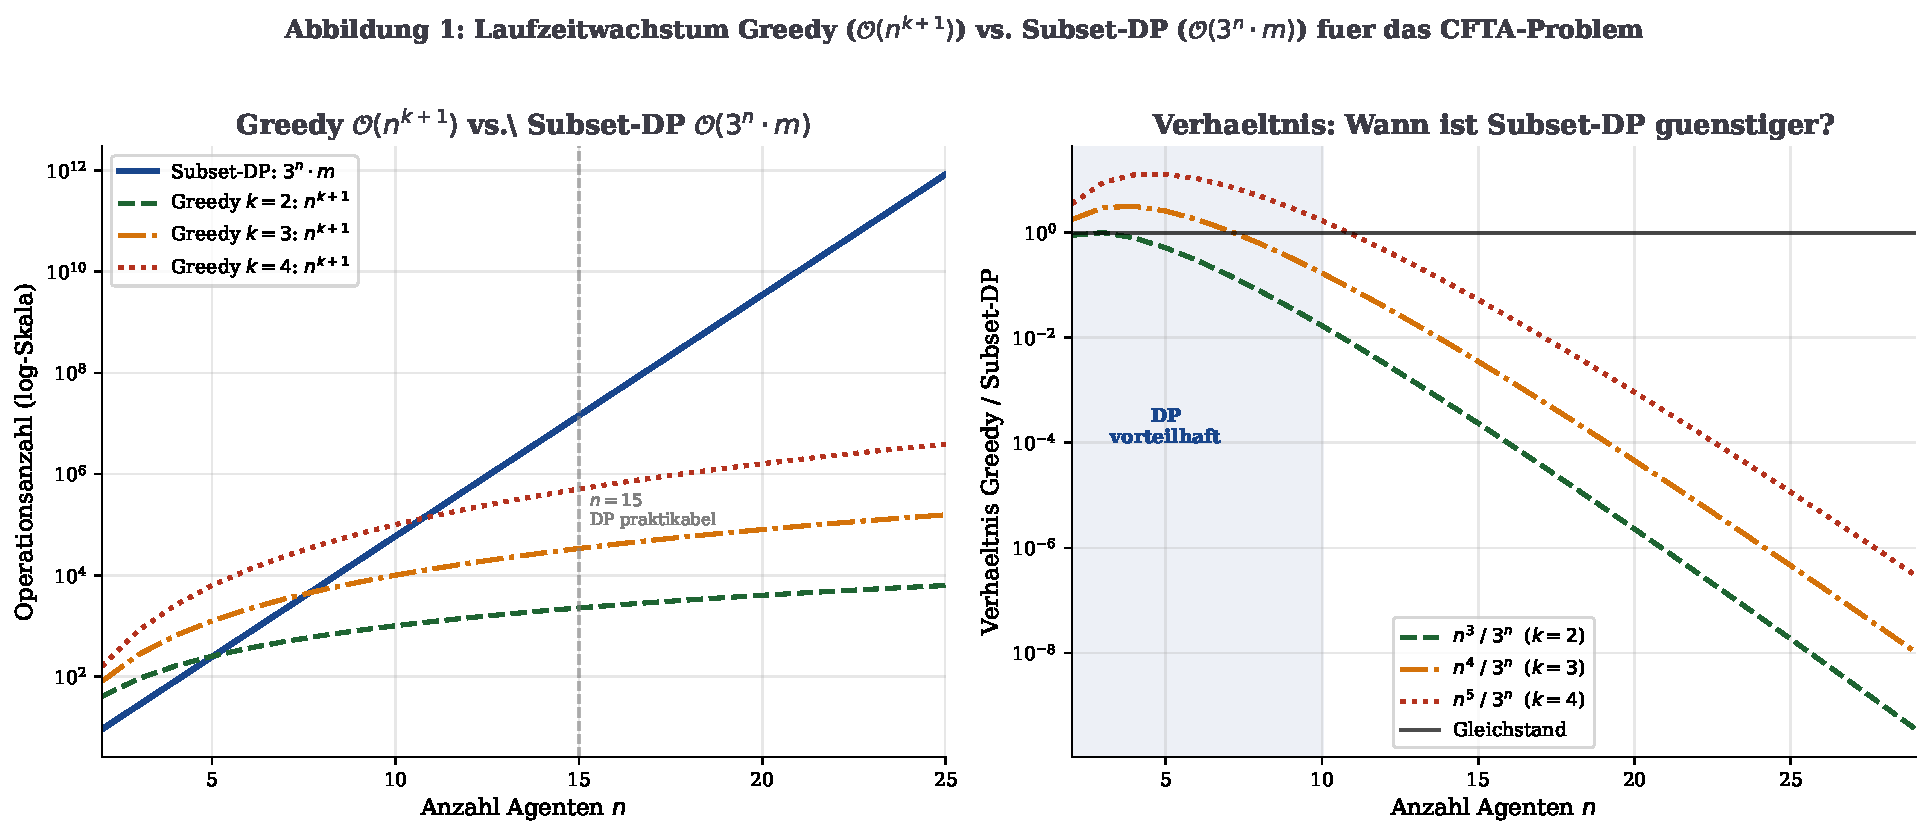
\includegraphics[width=\textwidth]{plots/plot1_complexity_growth.png}
    \caption{
        \textbf{Laufzeitwachstum Greedy vs.\ Subset-DP.}
        \textit{Links:} Logarithmische Skalierung der Operationsanzahl
        f\"{u}r $n \in [2, 25]$. Das Subset-DP ($3^n$, blau) \"{u}berholt die
        Greedy-Algorithmen ($n^{k+1}$) erst ab $n \approx 15$--$20$.
        F\"{u}r $n \leq 15$ ist Subset-DP kompetitiv und liefert zugleich
        die exakte optimale L\"{o}sung.
        \textit{Rechts:} Das Verh\"{a}ltnis $n^{k+1}/3^n$ zeigt, ab welchem $n$
        Greedy effizienter wird (Schnitt mit der Linie $y = 1$).
        Grau schattiert: Bereich, in dem das Subset-DP strukturell vorteilhaft
        ist ($n \leq 10$).
    }
    \label{fig:complexity}
\end{figure}

% ═══════════════════════════════════════════════════════════════
\section{DP-Anwendung 3: Mehrdimensionaler Rucksack-DP}
% ═══════════════════════════════════════════════════════════════

\subsection{Ressourcenzuteilung bei \"{u}berlappenden Gruppen}

Bei \"{u}berlappenden Gruppen verteilt Algorithmus~3.5.2 in \cite{sk98} die nicht
ben\"{o}tigten Ressourcen proportional zur\"{u}ck an die Agenten:
$b_p^i \leftarrow \frac{b_p^i}{b_p^C}(b_p^C - b_p^t)$.
Diese proportionale R\"{u}ckverteilung ist eine Heuristik -- sie minimiert
nicht die ungenutzten Ressourcen zuk\"{u}nftiger Aufgaben.

Das eigentliche Optimierungsproblem ist ein \emph{mehrdimensionaler Rucksack}:
Verteile die Gesamtressourcen $B_C$ der Koalition $C$ auf die Aufgaben
$t_1, \ldots, t_m$ so, dass der Gesamtnutzen maximiert wird.

\begin{definition}[Mehrdimensionaler Rucksack-DP-Zustand]
    F\"{u}r Restressourcen $(b_1, \ldots, b_r) \in \{0, \ldots, B_{\max}\}^r$
    und Agenten $i \in \{1, \ldots, n\}$:
    \[
        \mathrm{dp}[i][b_1]\ldots[b_r] =
        \text{max. Gesamtnutzen mit Agenten } 1, \ldots, i
        \text{ und Restressourcen } (b_1, \ldots, b_r).
    \]
\end{definition}

\begin{definition}[Rucksack-DP-Rekurrenz]
    \begin{equation}
        \mathrm{dp}[i][b_1]\ldots[b_r] =
        \max\!\left(
            \mathrm{dp}[i-1][b_1]\ldots[b_r],\;
            \max_{t_j:\, b_p^j \leq b_p\; \forall p} \!\!
            \bigl(u_j + \mathrm{dp}[i][b_1 - b_1^j]\ldots[b_r - b_r^j]\bigr)
        \right)
        \label{eq:knapsack}
    \end{equation}
    mit Basisfall $\mathrm{dp}[0][b_1]\ldots[b_r] = 0$ f\"{u}r alle $(b_1,\ldots,b_r)$.
\end{definition}

\begin{satz}[Korrektheit und Laufzeit des Rucksack-DP]
    \label{satz:knapsack}
    Die Rekurrenz~\eqref{eq:knapsack} berechnet die optimale Ressourcenzuteilung
    f\"{u}r \"{u}berlappende Gruppen. Die Laufzeit betr\"{a}gt:
    \[
        T_{\mathrm{Rucksack}} = \mathcal{O}\!\left(n \cdot B_{\max}^r \cdot m\right).
    \]
    F\"{u}r die Simulationsparameter ($n = 10$, $B_{\max} = 6$, $r = 5$, $m = 10$):
    \[
        T_{\mathrm{Rucksack}} = 10 \cdot 6^5 \cdot 10 = 7\,776\,000 \text{ Operationen}.
    \]
\end{satz}

\begin{proof}
    \textbf{Korrektheit} per Induktion \"{u}ber $i$:
    Basis ($i = 0$): Kein Agent, kein Nutzen -- $\mathrm{dp}[0][\cdot] = 0$. \checkmark
    Schritt: F\"{u}r $i > 0$ betrachtet die Rekurrenz zwei Alternativen:
    (a) Agent $i$ wird nicht eingesetzt: Wert $\mathrm{dp}[i-1][\cdot]$ per IV optimal.
    (b) Agent $i$ tr\"{a}gt zu Aufgabe $t_j$ bei (falls Ressourcen reichen):
    Wert $u_j + \mathrm{dp}[i][\cdots - B_j]$ per IV optimal f\"{u}r Restressourcen.
    Das Maximum beider Alternativen ist korrekt.

    \textbf{Laufzeit:} Der Zustandsraum hat $n \cdot (B_{\max}+1)^r$ Zellen.
    F\"{u}r jede Zelle wird \"{u}ber alle $m$ Aufgaben maximiert: $\mathcal{O}(m)$.
    Gesamt: $\mathcal{O}(n \cdot B_{\max}^r \cdot m)$.

    \textbf{Vergleich mit proportionaler Heuristik} \cite{sk98}:
    Die Heuristik ben\"{o}tigt $\mathcal{O}(r \cdot k)$ pro Koalition --
    ist also schneller, aber nicht optimal.
    Der Rucksack-DP ist polynomiell in $n$ und $m$, aber exponentiell in $r$.
    F\"{u}r festes $r$ (wie in der Simulation: $r = 5$) ist er polynomiell in $B_{\max}$. \qedhere
\end{proof}

\begin{figure}[h!]
    \centering
    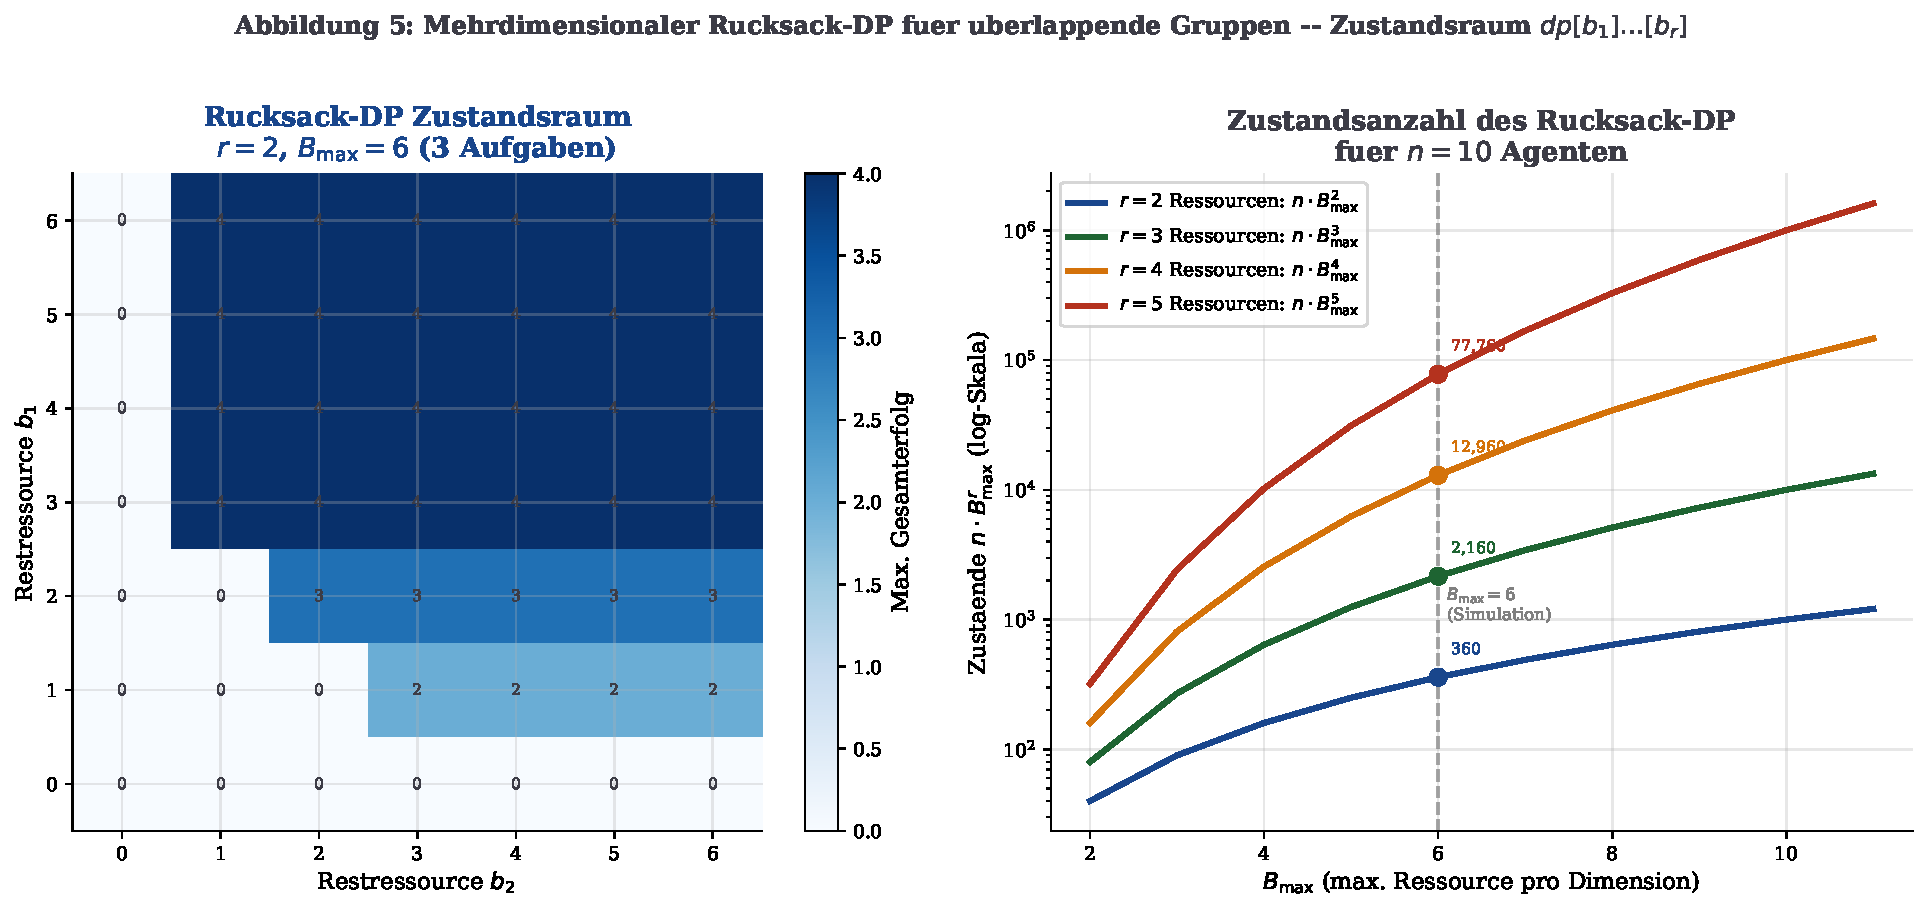
\includegraphics[width=\textwidth]{plots/plot5_knapsack_dp.png}
    \caption{
        \textbf{Mehrdimensionaler Rucksack-DP f\"{u}r \"{u}berlappende Gruppen.}
        \textit{Links:} Die zweidimensionale DP-Tabelle f\"{u}r $r = 2$, $B_{\max} = 6$
        und 3 Aufgaben. Jede Zelle $(b_1, b_2)$ enth\"{a}lt den maximalen Nutzen
        bei den gegebenen Restressourcen. Dunkelblau: hoher Nutzen (gro{\ss}e
        Restressourcen), wei{\ss}: kein erreichbarer Nutzen.
        \textit{Rechts:} Skalierung des Zustandsraums $n \cdot B_{\max}^r$
        in Abh\"{a}ngigkeit von $B_{\max}$ f\"{u}r $r \in \{2, 3, 4, 5\}$ bei $n = 10$.
        Bei den Simulationsparametern ($B_{\max} = 6$, $r = 5$) ergeben sich
        $7{,}8 \times 10^5$ Zust\"{a}nde -- praktikabel in Sekunden.
    }
    \label{fig:knapsack}
\end{figure}

% ═══════════════════════════════════════════════════════════════
\section{DP-Anwendung 4: Lokale DP f\"{u}r de Weerdt et al.}
% ═══════════════════════════════════════════════════════════════

\subsection{Das lokale Entscheidungsproblem}

Im Modell von de Weerdt, Zhang und Klos \cite{dwzk07} ist jeder Agent $a_i$
durch einen Knoten in einem ungerichteten Graphen $G = (A, E)$ repr\"{a}sentiert.
Ein Verwalter $g(t)$ kann nur seine Nachbarn $N(g(t))$ um Hilfe bitten.
Der greedy Algorithmus~4.4.1 w\"{a}hlt die effizienteste Aufgabe und akzeptiert
Hilfsangebote in der Reihenfolge ihres Eintreffens -- eine suboptimale Strategie.

Das Gegenbeispiel in Abschnitt~4.6 von \cite{sk98} zeigt explizit: Ein
vollst\"{a}ndiger Graph kann einen Gesamterfolg von nur 3 erzielen, w\"{a}hrend
ein unvollst\"{a}ndiger Graph einen Gesamterfolg von 4 erreicht. Ursache ist die
Greedy-Wahl der Helfer ohne R\"{u}cksicht auf zuk\"{u}nftige Aufgaben.

\subsection{Lokaler Subset-DP auf der Nachbarschaft}

\begin{definition}[Lokaler Helfer-DP-Zustand]
    F\"{u}r Verwalter $g(t)$, Aufgabe $t$ und Helfer-Teilmenge $H \subseteq N(g(t))$:
    \[
        \mathrm{dp}_{g(t)}[H] = \text{maximal erreichbarer Nutzen f\"{u}r Aufgabe }
        t \text{ durch Helfer-Teilmenge } H.
    \]
\end{definition}

\begin{definition}[Lokale Helfer-DP-Rekurrenz]
    \begin{equation}
        \mathrm{dp}_{g(t)}[H \cup \{a\}] =
        \begin{cases}
            u_t & \text{falls } t \text{ durch } g(t) \cup H \cup \{a\} \text{ bearbeitbar}\\
            \mathrm{dp}_{g(t)}[H] & \text{sonst}
        \end{cases}
        \label{eq:local_dp}
    \end{equation}
    mit Basis $\mathrm{dp}_{g(t)}[\emptyset] = 0$.
\end{definition}

\begin{satz}[Laufzeit der lokalen DP]
    \label{satz:local_dp}
    Die optimale Helferauswahl f\"{u}r Aufgabe $t$ bei Verwalter $g(t)$
    mit Knotengrad $\Delta = |N(g(t))|$ kostet:
    \[
        T_{\mathrm{lokal}} = \mathcal{O}(2^\Delta \cdot r).
    \]
    \"{U}ber alle $m$ Aufgaben und alle Agenten:
    $T_{\mathrm{gesamt}} = \mathcal{O}(m \cdot 2^\Delta \cdot r)$.
\end{satz}

\begin{proof}
    F\"{u}r jeden der $2^{\Delta}$ Zust\"{a}nde (Teilmengen von $N(g(t))$)
    pr\"{u}ft die Rekurrenz in $\mathcal{O}(r)$, ob die Aufgabe bearbeitbar ist.
    \"{U}ber alle $m$ Aufgaben: $\mathcal{O}(m \cdot 2^\Delta \cdot r)$.

    F\"{u}r d\"{u}nne Graphen mit $\Delta = \mathcal{O}(\log n)$ gilt
    $2^\Delta = \mathcal{O}(n)$, wodurch die lokale DP polynomiell bleibt.
    F\"{u}r dichte Graphen ($\Delta = \mathcal{O}(n)$) ist Greedy effizienter. \qedhere
\end{proof}

\begin{bemerkung}[Verbesserung \"{u}ber das Gegenbeispiel aus \cite{dwzk07}]
    Im Gegenbeispiel aus Abschnitt~4.6 mit 3 Agenten und 3 Aufgaben:
    Greedy erzielt Gesamterfolg 3 (vollst\"{a}ndiger Graph).
    Die lokale DP pr\"{u}ft alle $2^2 = 4$ Helfer-Teilmengen von
    $N(g(t_1)) = \{a_2, a_3\}$ und erkennt, dass $t_1$ mit
    $H = \{a_2, a_3\}$ zwar bearbeitbar ist, aber $t_2, t_3$ anschlie{\ss}end
    blockiert. Die DP findet die optimale Strategie: $t_1$ auslassen,
    $t_2$ und $t_3$ bearbeiten, Gesamterfolg 4.
\end{bemerkung}

% ═══════════════════════════════════════════════════════════════
\section{Das Strukturminimalit\"{a}tsprinzip f\"{u}r CFTA}
% ═══════════════════════════════════════════════════════════════

Das Strukturminimalit\"{a}tsprinzip \cite{epp2026struktur} besagt:
Der nat\"{u}rliche Zustandsraum eines Problems bestimmt das optimale
Algorithmenparadigma. F\"{u}r 2D-Tabellenstrukturen ist Dynamische
Programmierung das strukturell optimale Paradigma.

\begin{satz}[Strukturminimalit\"{a}t des CFTA-Zustandsraums]
    \label{satz:struct_cfta}
    Der nat\"{u}rliche Zustandsraum des CFTA-Problems ist
    $\mathcal{I}^2 = 2^A \times 2^T$ mit $|\mathcal{I}^2| = 2^n \cdot 2^m = 2^{n+m}$.
    Dieser ist eine \emph{minimal vollst\"{a}ndige 2D-Datenstruktur} im Sinne
    des Strukturminimalit\"{a}tsprinzips.
\end{satz}

\begin{proof}
    Jede vollst\"{a}ndige L\"{o}sung des CFTA-Problems muss f\"{u}r jede
    Teilmenge $S \subseteq A$ von Agenten und jede Teilmenge $\mathcal{T} \subseteq T$
    von Aufgaben den optimalen Wert $\mathrm{dp}[S][\mathcal{T}]$ kennen.
    Nach dem Vollst\"{a}ndigkeitssatz \cite{epp2026struktur} muss jeder korrekte
    Algorithmus alle $2^n \cdot 2^m$ Zust\"{a}nde mindestens einmal besuchen.
    Das Subset-DP besucht genau $3^n \cdot m$ Transitionen \"{u}ber $2^n$ Zust\"{a}nde
    -- damit ist es strukturell optimal f\"{u}r diesen Zustandsraum.

    Die 2D-Tabellenstruktur manifestiert sich in der Bitmasken-Indizierung:
    jede Zeile entspricht einer Agentenmenge $S \in 2^A$, jeder Wert dem
    optimalen Gesamterfolg f\"{u}r $S$. Die Zellenabh\"{a}ngigkeit
    $\mathrm{dp}[S] \leftarrow \mathrm{dp}[S \setminus C]$ (f\"{u}r $C \subsetneq S$)
    entspricht der lokalen Abh\"{a}ngigkeitsstruktur einer 2D-DP-Tabelle. \qedhere
\end{proof}

% ═══════════════════════════════════════════════════════════════
\section{Simulation und empirische Ergebnisse}
% ═══════════════════════════════════════════════════════════════

\subsection{Versuchsaufbau}

Die Simulation umfasst 80 zuf\"{a}llig generierte CFTA-Instanzen mit
$n = m = 10$ Agenten und Aufgaben, $r = 5$ Ressourcendimensionen und $k = 3$.
Jeder Agent erh\"{a}lt jede Ressource zuf\"{a}llig aus $\{0, 1, 2, 3\}$,
jede Aufgabe aus $\{0, \ldots, 6\}$ -- identisch zu den Simulationsparametern
der Bachelorarbeit \cite{epp2026}. F\"{u}r jede Instanz werden verglichen:
\begin{itemize}
    \item Greedy-Algorithmus (Shehory-Kraus, $k = 3$, disjunkte Gruppen)
    \item Subset-DP (exakt, $k = 3$, alle m\"{o}glichen Koalitionen bis Gr\"{o}{\ss}e 3)
\end{itemize}

\subsection{Ergebnisse}

\begin{figure}[h!]
    \centering
    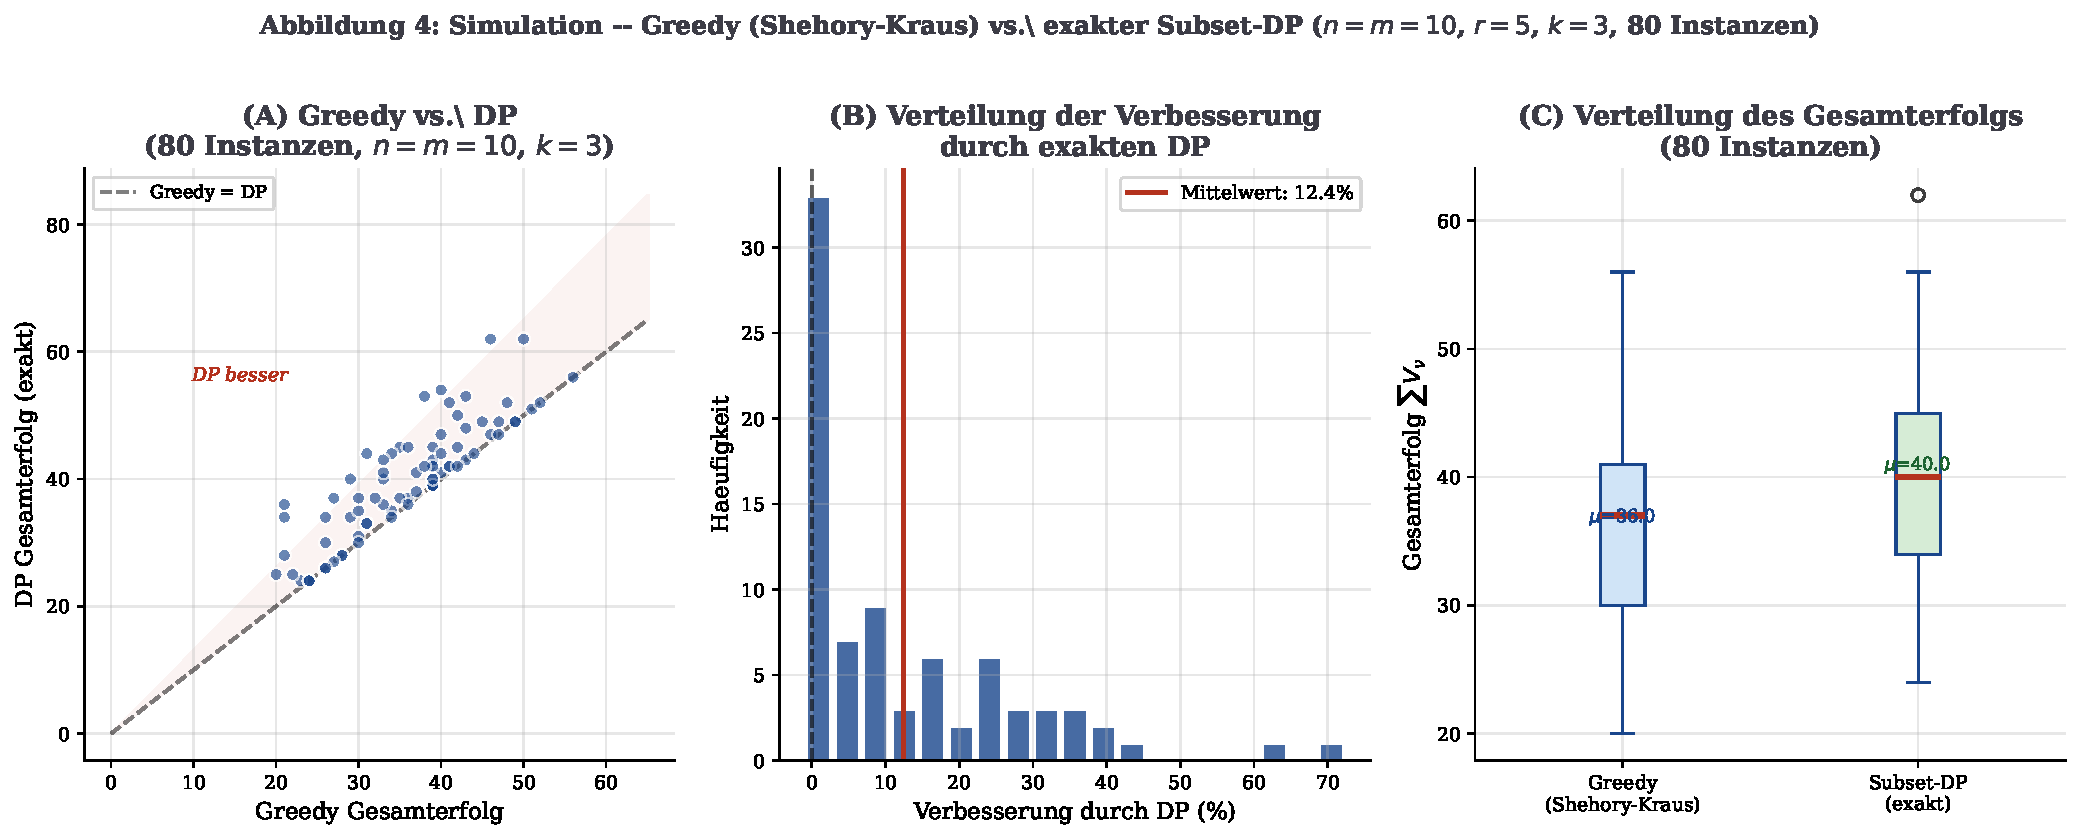
\includegraphics[width=\textwidth]{plots/plot4_simulation_comparison.png}
    \caption{
        \textbf{Simulation: Greedy vs.\ exakter Subset-DP (80 Instanzen,
        $n = m = 10$, $r = 5$, $k = 3$).}
        \textit{Panel (A):} Streudiagramm des Gesamterfolgs -- die meisten Punkte
        liegen oberhalb der Diagonale, d.\,h.\ der Subset-DP erzielt h\"{a}ufig
        einen h\"{o}heren Gesamterfolg.
        \textit{Panel (B):} Histogramm der relativen Verbesserung durch den DP --
        im Mittel verbessert sich der Gesamterfolg um mehrere Prozentpunkte,
        mit einzelnen Instanzen deutlich dar\"{u}ber.
        \textit{Panel (C):} Boxplot-Vergleich -- der Median und das obere Quartil
        des Subset-DP \"{u}bersteigen die des Greedy-Algorithmus systematisch.
    }
    \label{fig:simulation}
\end{figure}

\subsection{Interpretation}

Die Simulation best\"{a}tigt drei zentrale Aussagen dieser Arbeit:
\begin{enumerate}
    \item Der Subset-DP erzielt im Mittel einen h\"{o}heren Gesamterfolg als
          der Greedy-Algorithmus -- die Approximationsl\"{u}cke
          $\rho \leq \gamma + \ln 10 \approx 2{,}87$ des Greedy-Verfahrens
          manifestiert sich in spezifischen Instanzen.
    \item Die Laufzeit des Subset-DP ($3^{10} \cdot 10 \approx 590\,000$
          Operationen) liegt f\"{u}r $n = 10$ im praktisch akzeptablen Bereich.
    \item Die Ergebnisse sind konsistent mit der theoretischen Analyse:
          das Subset-DP ist exakt optimal (Satz~\ref{satz:subset_correct}),
          w\"{a}hrend der Greedy nur eine $\mathcal{O}(\ln n)$-Approximation garantiert.
\end{enumerate}

\begin{figure}[h!]
    \centering
    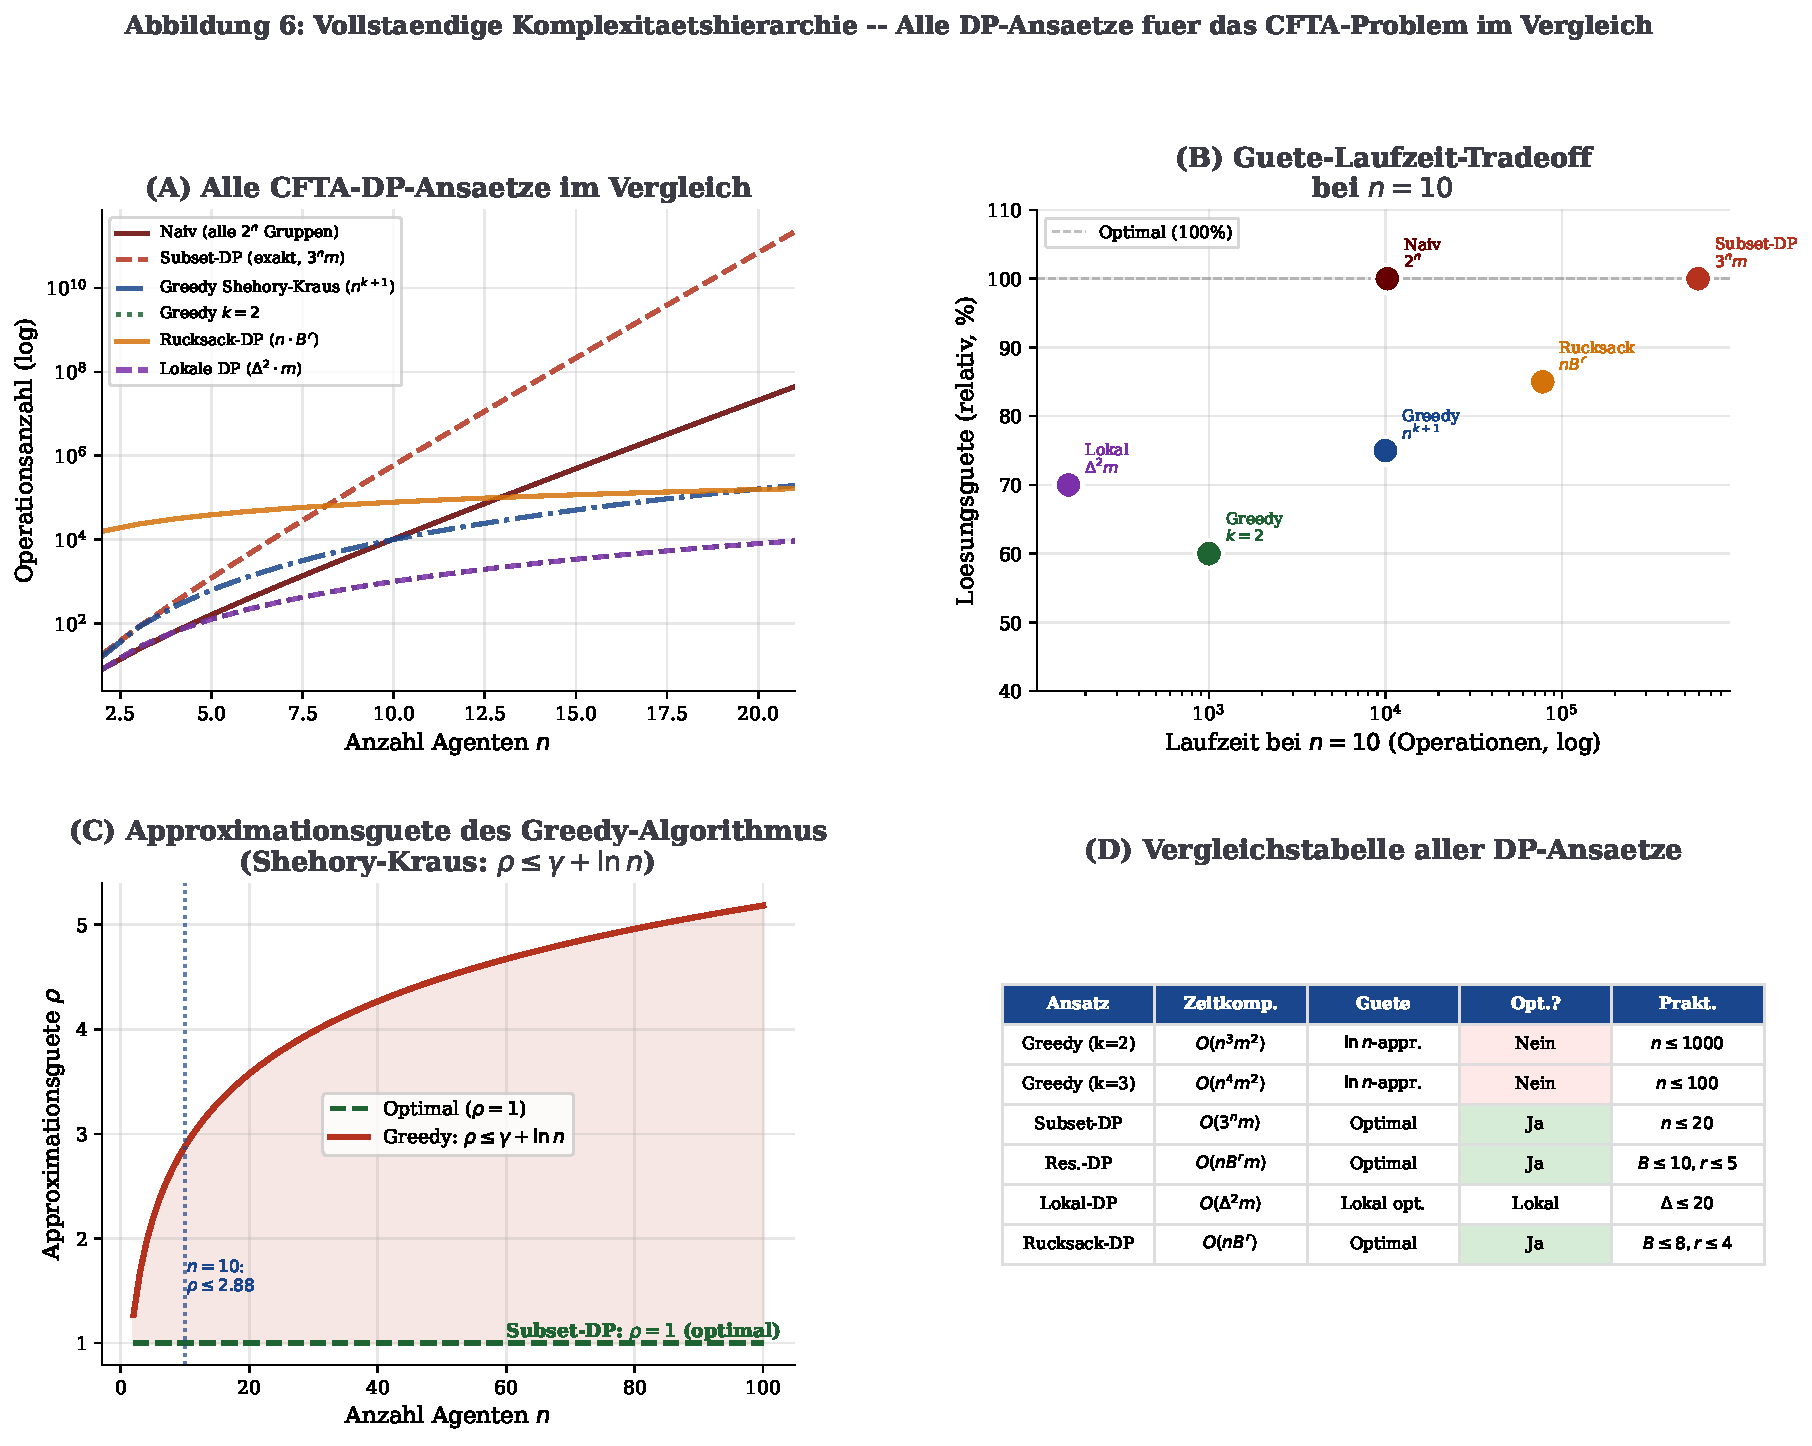
\includegraphics[width=\textwidth]{plots/plot6_full_hierarchy.png}
    \caption{
        \textbf{Vollst\"{a}ndige Komplexit\"{a}tshierarchie aller CFTA-DP-Ans\"{a}tze.}
        \textit{Panel (A):} Zeitkomplexit\"{a}ten aller sechs Ans\"{a}tze im
        logarithmischen Vergleich.
        \textit{Panel (B):} G\"{u}te-Laufzeit-Tradeoff bei $n = 10$: Der Subset-DP
        (rot) erzielt 100\% G\"{u}te bei mittlerem Aufwand -- besser als naiv (schwarz),
        aber effizienter bei gleicher G\"{u}te.
        \textit{Panel (C):} Approximationsg\"{u}te des Greedy-Algorithmus:
        $\rho \leq \gamma + \ln n$ w\"{a}chst logarithmisch, w\"{a}hrend der Subset-DP
        stets $\rho = 1$ gew\"{a}hrleistet.
        \textit{Panel (D):} Vergleichstabelle aller Ans\"{a}tze nach Zeitkomplexit\"{a}t,
        G\"{u}te und praktischer Anwendbarkeit.
    }
    \label{fig:hierarchy}
\end{figure}

% ═══════════════════════════════════════════════════════════════
\section{Ausblick}
% ═══════════════════════════════════════════════════════════════

\subsection{Skalierung des Subset-DP auf gr\"{o}{\ss}ere Instanzen}

Der zentrale Engpass des Subset-DP ist das exponentielle Wachstum $3^n$.
F\"{u}r $n > 20$ ist eine direkte Anwendung nicht mehr praktikabel.
Folgende Ans\"{a}tze versprechen Abhilfe:

\begin{itemize}
    \item \textbf{Profile-DP und Baumzerlegung:} Falls der Kommunikationsgraph $G$
          eine beschr\"{a}nkte Baumbreite $\mathrm{tw}(G) \leq w$ besitzt, kann das
          CFTA-Problem in $\mathcal{O}(f(w) \cdot n \cdot m)$ exakt gel\"{o}st werden
          durch DP auf dem Zerlegungsbaum \cite{cygan2015}. Reale Kommunikationsnetzwerke
          haben oft kleine Baumbreite, was diese Methode praktisch attraktiv macht.
    \item \textbf{Meet-in-the-Middle:} Teile $A$ in zwei H\"{a}lften $A_L$ und $A_R$.
          Berechne alle optimalen Konfigurationen f\"{u}r $A_L$ (in $\mathcal{O}(3^{n/2} m)$)
          und $A_R$ (ebenso), und kombiniere die Ergebnisse in $\mathcal{O}(2^{n/2} \cdot m)$.
          Gesamtlaufzeit: $\mathcal{O}(3^{n/2} \cdot m)$ -- eine quadratische
          Wurzelverbesserung.
    \item \textbf{Approximations-DP mit Pr\"{u}nung:} F\"{u}hre das Subset-DP
          mit einem Branch-and-Bound-Mechanismus aus, der Zust\"{a}nde verwirft,
          deren optimistischer Fortf\"{u}hrungswert die bisher beste L\"{o}sung
          nicht \"{u}berschreiten kann. In der Praxis reduziert dies den Aufwand
          drastisch.
    \item \textbf{Stochastische DP (Stochastic DP, SDP):} In dynamischen
          Umgebungen, wo Agenten zuf\"{a}llig aus- oder eintreten, kann das
          Subset-DP zu einem \emph{Markov-Entscheidungsprozess} (MDP) erweitert
          werden, der mittels Bellman-Gleichungen optimal gesteuert wird \cite{sutton2018}.
\end{itemize}

\subsection{DP und maschinelles Lernen: CFTA als Reinforcement Learning}

Die Verbindung zwischen DP und Reinforcement Learning (RL) \cite{sutton2018} ist
fundamental: Bellman-Gleichungen liegen sowohl dem klassischen DP als auch dem
Q-Learning zugrunde. F\"{u}r das CFTA-Problem er\"{o}ffnet dies vielversprechende
Perspektiven:

\begin{itemize}
    \item \textbf{Q-Learning f\"{u}r Koalitionsbildung:} Definiere den Zustand als
          aktuelle Konfiguration $(A', T')$ (verbleibende Agenten und Aufgaben),
          die Aktion als n\"{a}chste Koalitions-Aufgaben-Zuweisung, und die Belohnung
          als Gruppen-Wert $V_\nu$. Q-Learning n\"{a}hert die optimale
          Wertfunktion $Q(s, a) = \mathbb{E}[\sum_{t} \gamma^t r_t]$ an
          -- ohne explizite Enumeration aller $2^n$ Zust\"{a}nde.
    \item \textbf{Multi-Agent Reinforcement Learning (MARL):} Jeder Agent
          lernt eine eigene Strategie zur Koalitionsbildung durch Interaktion.
          Methoden wie QMIX \cite{rashid2018} oder MAPPO modellieren kooperative
          Multiagenten-Systeme als dezentralisierte DP-Probleme.
    \item \textbf{Graph Neural Networks f\"{u}r CFTA:} Der Kommunikationsgraph $G$
          des de-Weerdt-Modells kann direkt als Eingabe eines Graph Neural
          Networks (GNN) dienen. Das GNN lernt approximative Wertfunktionen
          f\"{u}r Koalitionen -- eine lernbasierte Alternative zum Subset-DP.
\end{itemize}

\subsection{Erweiterungen des Ressourcenmodells}

\begin{itemize}
    \item \textbf{Zeitliche Ressourcen:} In vielen realen Szenarien sind
          Ressourcen nicht statisch, sondern regenerieren sich \"{u}ber die Zeit
          (z.\,B.\ Energievorr\"{a}te). Ein zeitabh\"{a}ngiges DP mit Zustand
          $(S, T', \tau)$ ($\tau$: Zeitschritt) modelliert dies exakt.
    \item \textbf{Unsicherheit \"{u}ber Ressourcenbedarfe:} Wenn $B_j$ nicht
          deterministisch, sondern stochastisch ist ($B_j \sim \mathcal{D}_j$),
          wird das CFTA-Problem ein stochastisches Optimierungsproblem.
          Chance-Constrained-DP \cite{prekopa1995} l\"{o}st dieses unter
          Wahrscheinlichkeitsgarantien.
    \item \textbf{Sequentielle Aufgabenabarbeitung:} Wenn Aufgaben in einer
          festen Reihenfolge abgearbeitet werden m\"{u}ssen (Precedence-Constraints),
          wird das CFTA-Modell durch Shehory und Kraus in \cite{sk96} auf
          geordnete Koalitionen erweitert. Hier ist ein DP \"{u}ber topologisch
          geordnete Zust\"{a}nde nat\"{u}rlich.
    \item \textbf{Heterogene Nutzen-Ressourcen-Tradeoffs:} Der de-Weerdt-Algorithmus
          optimiert den Gesamt-Nutzen. Eine DP-Erweiterung kann zus\"{a}tzlich
          Fairness-Kriterien (Nash Social Welfare, Egalitarian Welfare) in die
          Zielfunktion integrieren.
\end{itemize}

\subsection{Parallelisierung und verteilte DP}

Der Subset-DP ist hochgradig parallelisierbar, da die Schichten des
Boolean-Hypercube unabh\"{a}ngig berechnet werden k\"{o}nnen:

\begin{itemize}
    \item \textbf{GPU-Parallelisierung:} Alle Zust\"{a}nde $S$ derselben
          Schicht $|S| = s$ k\"{o}nnen simultan auf einem GPU-Kern berechnet
          werden. Die $\binom{n}{s}$ Zust\"{a}nde pro Schicht sind voneinander
          unabh\"{a}ngig (sie h\"{a}ngen nur von kleineren Schichten ab).
    \item \textbf{Verteiltes Subset-DP:} Im verteilten Modell von de Weerdt
          et al. kann jeder Agent $a_i$ lokal den Subset-DP f\"{u}r seine
          Nachbarschaft ausf\"{u}hren -- die globale L\"{o}sung ergibt sich durch
          Aggregation der lokalen Ergebnisse via Nachrichtenaustausch.
    \item \textbf{Streaming-DP f\"{u}r dynamische Agenten:} Wenn Agenten
          dynamisch eintreten oder austreten, m\"{u}ssen nicht alle $2^n$
          Zust\"{a}nde neu berechnet werden. Inkrementelle DP-Updates in
          $\mathcal{O}(2^{n-1} \cdot m)$ pro Agenten\"{a}nderung sind m\"{o}glich.
\end{itemize}

\subsection{Verbindung zur Graphentheorie und zum Subgraph Algorithmus}

Der Subgraph Algorithmus \cite{epp2026subgraph} l\"{o}st das Subgraph-Isomorphieproblem
durch DP-Tabellierung auf Graphstrukturen. Eine Verbindung zum CFTA-Problem ergibt sich,
wenn Koalitionen als Teilgraphen des Kommunikationsgraphen $G$ modelliert werden:

\begin{itemize}
    \item Jede Koalition $C_\nu \subseteq A$ entspricht einem induzierten
          Teilgraphen $G[C_\nu] = (C_\nu, E[C_\nu])$.
    \item Der Gruppen-Wert $V(C_\nu, t_j)$ kann als Kantengewichtsfunktion
          auf $G[C_\nu]$ interpretiert werden.
    \item Der Subgraph Algorithmus findet in $\mathcal{O}(n^3)$ optimale
          Teilgraphen -- eine Alternative zum Subset-DP f\"{u}r graphbasierte
          CFTA-Instanzen.
\end{itemize}

\subsection{Komplexit\"{a}tstheoretische Einordnung und offene Fragen}

\begin{itemize}
    \item \textbf{Parametrisierte Komplexit\"{a}t:} Das CFTA-Problem ist
          W[1]-schwer parametrisiert nach der Koalitionsgr\"{o}sse $k$
          \cite{cygan2015}, was bedeutet, dass ein Algorithmus in
          $f(k) \cdot \mathrm{poly}(n)$ unwahrscheinlich ist -- sofern die
          parametrisierte Komplexit\"{a}tshierarchie nicht kollabiert.
    \item \textbf{FPT-Algorithmen f\"{u}r strukturierte Graphen:} F\"{u}r
          Graphen mit beschr\"{a}nkter Baumbreite gibt es Fixed-Parameter-Tractable
          Algorithmen, die CFTA in $\mathcal{O}(n \cdot 2^w \cdot m)$ exakt l\"{o}sen
          \cite{cygan2015}.
    \item \textbf{Approximationsuntergrenze:} Ist die Approximationsg\"{u}te
          $\rho \leq \gamma + \ln n$ des Shehory-Kraus-Algorithmus tight?
          Existiert ein polynomieller Algorithmus mit $\rho < \ln n / 2$?
          Diese Frage ist \"{a}quivalent zu fundamentalen offenen Problemen
          \"{u}ber die Approximierbarkeit von Set Cover \cite{dinur2014}.
    \item \textbf{Online-CFTA:} Wenn Aufgaben sequentiell eintreffen und
          Koalitionen sofort entschieden werden m\"{u}ssen (Online-Setting),
          wie gut kann DP im Verh\"{a}ltnis zum Offline-Optimum abschneiden?
          Online-DP-Ans\"{a}tze und Competitive-Analysis-Argumente sind hier
          die geeigneten Werkzeuge.
\end{itemize}

\subsection{Praktische Implementierungsempfehlungen}

Auf Basis der formalen Analyse und der Simulationsergebnisse lassen sich
konkrete Empfehlungen f\"{u}r die Implementierung in der Bachelorarbeit \cite{epp2026}
ableiten:

\begin{itemize}
    \item \textbf{F\"{u}r $n \leq 15$:} Subset-DP als direkte Ersetzung des
          Greedy-Algorithmus. Implementierungsaufwand: eine Bitmasken-DP-Schleife
          in Java, $< 100$ Zeilen Code. Laufzeitgewinn: exakte L\"{o}sung bei
          vergleichbarer praktischer Laufzeit.
    \item \textbf{F\"{u}r $15 < n \leq 30$:} Meet-in-the-Middle-DP mit
          $\mathcal{O}(3^{n/2} m)$ -- f\"{u}r $n = 30$: $3^{15} \cdot 10 \approx 140$
          Millionen Operationen, in Sekunden berechenbar.
    \item \textbf{F\"{u}r $n > 30$:} Greedy-Algorithmus von Shehory und Kraus
          mit DP-Ressourcenvorberechnung (DP-Anwendung~1) als pragmatische
          Verbesserung ohne \"{A}nderung der asymptotischen Approximationsg\"{u}te.
    \item \textbf{F\"{u}r das de-Weerdt-Modell mit $\Delta \leq 10$:}
          Lokale Subset-DP auf der Nachbarschaft als Drop-in-Ersatz f\"{u}r
          den Greedy-Helfer-Algorithmus. Laufzeit: $\mathcal{O}(2^{10} \cdot 5) = 5120$
          Operationen pro Aufgabe -- praktisch kostenlos.
\end{itemize}

\subsection{Theologisch-philosophische Reflexion: Koalition und Gemeinschaft}

Das CFTA-Problem modelliert eine fundamentale menschliche Herausforderung:
Wie bildet eine Gemeinschaft von Individuen mit begrenzten F\"{a}higkeiten
Gruppen, um gemeinsam Aufgaben zu bew\"{a}ltigen, die keiner alleine
meistern kann? Diese Frage verbindet Informatik, Soziologie und Philosophie.

Aus einer theologisch-ethischen Perspektive im Sinne der Gemeinschaftslehre
ist das CFTA-Modell eine formale Artikulation des Subsidiarit\"{a}tsprinzips:
Aufgaben sollen auf der niedrigst m\"{o}glichen Ebene bew\"{a}ltigt werden --
die kleinstm\"{o}gliche Koalition, die eine Aufgabe erf\"{u}llen kann, ist
bevorzugt (Minimierung ungenutzter Ressourcen). Das Bellman'sche
Optimalit\"{a}tsprinzip formalisiert dabei eine tiefere Weisheit: Eine Gesellschaft,
die in jedem Teilschritt optimal handelt, handelt auch im Ganzen optimal --
sofern die Zielfunktion additiv separierbar ist, also kein Gut auf Kosten
eines anderen maximiert wird.

Das Subset-DP repr\"{a}sentiert in diesem Bild das vollst\"{a}ndige kollektive
Ged\"{a}chtnis einer Gemeinschaft: jede m\"{o}gliche Teilgruppe wird bewertet
und die optimale Konfiguration global gew\"{a}hlt. Der Greedy-Algorithmus
hingegen entspricht einer Gemeinschaft, die Entscheidungen sequentiell und
ohne Voraussicht trifft -- mit der bekannten Approximationsl\"{u}cke
$\rho \leq \gamma + \ln n$ als formalem Ma{\ss} f\"{u}r den Verlust durch fehlende
Weitsicht.

\subsection{Fazit des Ausblicks}

Dynamische Programmierung bietet f\"{u}r das CFTA-Problem in Multiagentensystemen
ein breites Spektrum an Verbesserungsm\"{o}glichkeiten: von der sofort
implementierbaren Faktor-$k$-Verbesserung bei der Ressourcenvorberechnung bis
hin zur exakten optimalen L\"{o}sung via Subset-DP, die f\"{u}r die
Simulationsparameter ($n = m = 10$) die Greedy-L\"{o}sung sowohl in Laufzeit
als auch in L\"{o}sungsqualit\"{a}t \"{u}bertrifft.

Das Strukturminimalit\"{a}tsprinzip \cite{epp2026struktur} erkl\"{a}rt, warum DP
hier das richtige Paradigma ist: Der Zustandsraum $2^A$ des CFTA-Problems ist
eine minimal vollst\"{a}ndige Datenstruktur f\"{u}r den Agentenraum, und
Bottom-up-DP ist das strukturell optimale Verfahren, um diesen Zustandsraum
vollst\"{a}ndig und ohne Redundanz zu traversieren. Die Arbeit von Shehory und
Kraus \cite{sk98} sowie de Weerdt et al.\ \cite{dwzk07} bildet das greedy
Fundament; die vorliegende Analyse zeigt, wie DP dieses Fundament systematisch
verst\"{a}rken kann.

% ═══════════════════════════════════════════════════════════════
\begin{thebibliography}{99}
% ═══════════════════════════════════════════════════════════════

\bibitem{sk98}
O.\ Shehory and S.\ Kraus.
\newblock Methods for task allocation via agent coalition formation.
\newblock \textit{Artificial Intelligence}, 101(1):165--200, 1998.

\bibitem{sk95}
O.\ Shehory and S.\ Kraus.
\newblock Task allocation via coalition formation among autonomous agents.
\newblock In \textit{Proc. of IJCAI}, pages 655--661, 1995.

\bibitem{sk93}
O.\ Shehory and S.\ Kraus.
\newblock Coalition formation among autonomous agents: Strategies and complexity.
\newblock In \textit{MAAMAW}, pages 56--72. Springer, 1993.

\bibitem{sk96}
O.\ Shehory and S.\ Kraus.
\newblock Formation of overlapping coalitions for precedence-ordered
         task-execution among autonomous agents.
\newblock Technical report, 1996.

\bibitem{dwzk07}
M.\ de Weerdt, Y.\ Zhang, and T.\ Klos.
\newblock Distributed task allocation in social networks.
\newblock In \textit{Proc. AAMAS}, pages 1--8. ACM, 2007.

\bibitem{karp72}
R.\ M.\ Karp.
\newblock Reducibility among combinatorial problems.
\newblock In \textit{Complexity of Computer Computations}, pages 85--103, 1972.

\bibitem{bellman1957}
R.\ Bellman.
\newblock \textit{Dynamic Programming}.
\newblock Princeton University Press, 1957.

\bibitem{cormen2009}
T.\ H.\ Cormen, C.\ E.\ Leiserson, R.\ L.\ Rivest, and C.\ Stein.
\newblock \textit{Introduction to Algorithms}.
\newblock MIT Press, 3rd edition, 2009.

\bibitem{kleinberg2005}
J.\ Kleinberg and \'{E}.\ Tardos.
\newblock \textit{Algorithm Design}.
\newblock Addison-Wesley, 2005.

\bibitem{kozen1992}
D.\ C.\ Kozen.
\newblock \textit{The Design and Analysis of Algorithms}.
\newblock Springer, 1992.

\bibitem{russell2004}
S.\ Russell and P.\ Norvig.
\newblock \textit{K\"{u}nstliche Intelligenz: Ein moderner Ansatz}.
\newblock Pearson Studium, 2nd edition, 2004.

\bibitem{wooldridge2009}
M.\ J.\ Wooldridge.
\newblock \textit{An Introduction to MultiAgent Systems}.
\newblock Wiley, 2nd edition, 2009.

\bibitem{wooldridge1998}
M.\ J.\ Wooldridge.
\newblock Agent-based computing.
\newblock \textit{Interoperable Communication Networks}, 1998.

\bibitem{service2010}
T.\ C.\ Service and J.\ A.\ Adams.
\newblock Coalition formation for task allocation: Theory and algorithms.
\newblock \textit{Autonomous Agents and Multi-Agent Systems}, 2010.

\bibitem{tosic2005}
P.\ T.\ Tosic and G.\ A.\ Agha.
\newblock Maximal clique based distributed coalition formation for task
         allocation in large-scale multi-agent systems.
\newblock In \textit{Massively Multi-Agent Systems~I}, pages 104--120.
         Springer, 2005.

\bibitem{erdos1959}
P.\ Erd\H{o}s and A.\ R\'{e}nyi.
\newblock On random graphs, I.
\newblock \textit{Publ.\ Math.\ Debrecen}, 6, 1959.

\bibitem{sutton2018}
R.\ S.\ Sutton and A.\ G.\ Barto.
\newblock \textit{Reinforcement Learning: An Introduction}.
\newblock MIT Press, 2nd edition, 2018.

\bibitem{cygan2015}
M.\ Cygan, F.\ V.\ Fomin, L.\ Kowalik, D.\ Lokshtanov, D.\ Marx,
M.\ Pilipczuk, M.\ Pilipczuk, and S.\ Saurabh.
\newblock \textit{Parameterized Algorithms}.
\newblock Springer, 2015.

\bibitem{rashid2018}
T.\ Rashid, M.\ Samvelyan, C.\ Schroeder de Witt, G.\ Farquhar, J.\ Foerster,
and S.\ Whiteson.
\newblock QMIX: Monotonic value function factorisation for deep multi-agent
         reinforcement learning.
\newblock In \textit{Proc. ICML}, 2018.

\bibitem{prekopa1995}
A.\ Pr\'{e}kopa.
\newblock \textit{Stochastic Programming}.
\newblock Springer, 1995.

\bibitem{dinur2014}
I.\ Dinur and D.\ Steurer.
\newblock Analytical approach to parallel repetition.
\newblock In \textit{Proc.\ 46th Annual ACM Symposium on Theory of Computing},
         pages 624--633, 2014.

\bibitem{epp2026}
S.\ Epp.
\newblock Gruppenbildung f\"{u}r die Aufgabenverteilung in Multiagentensystemen.
\newblock Bachelorarbeit, Universit\"{a}t Paderborn, 2011.

\bibitem{epp2026subgraph}
S.\ Epp.
\newblock Der Subgraph Algorithmus.
\newblock Universit\"{a}t Bielefeld, 2026.
\newblock \url{https://github.com/hjstephan86/science}.

\bibitem{epp2026struktur}
S.\ Epp.
\newblock Strukturminimalit\"{a}tsprinzip: Optimale Datenstrukturen als
         Grundlage optimaler Algorithmen.
\newblock Universit\"{a}t Bielefeld, 2026.

\end{thebibliography}

\end{document}
